\documentclass[10pt]{article}
\usepackage{graphicx}
\usepackage{amssymb}
\usepackage[fleqn]{amsmath}
\usepackage{nccmath}
\usepackage{cases}
\usepackage{hyperref}
\usepackage{multicol}
\usepackage{tikz}
\usepackage{pgfplots}
\usepackage{enumitem}
\pgfplotsset{compat=1.18}
\usepackage{float}
\usepackage{pdfpages}

\title{\bf Math 116: Worksheet 4}
\date{2/8/2024}
\author{\bf Owen Jones}
\begin{document}
\maketitle
\begin{enumerate}[label= \arabic*.]
    \item I used pow($18491332,2,20979031$) and checked it was equal to $43^2$.
    \item \begin{enumerate}
        \item From Euclid's lemma, if $p\mid (x-3)(x+3)$ then $p\mid (x-3)$ or $p\mid (x+3)$. Thus, $x\equiv \pm3\pmod{p}$.
        \item $x=459$
    \end{enumerate}
    \item Suppose $x^2\equiv y^2\pmod{n}$. It follows $x^2\equiv y^2\pmod{a}$ and $x^2\equiv y^2\pmod{b}$. 
    Thus, $x\equiv \pm y\pmod{a}$ and $x\equiv \pm y\pmod{b}$.
    Choose $x$ s.t $x\equiv y\pmod{a}$ and $x\equiv-y\pmod{b}$.
    Thus, $x\not\equiv \pm y\pmod{n}$ because we have either $x\equiv y\pmod{a}$ or $x\equiv-y\pmod{b}$.
    \item It passes for all except $7$. Definitely composite.
    \item Fails to pass Miller Rabin $a=3$. $5197$ is a factor.
    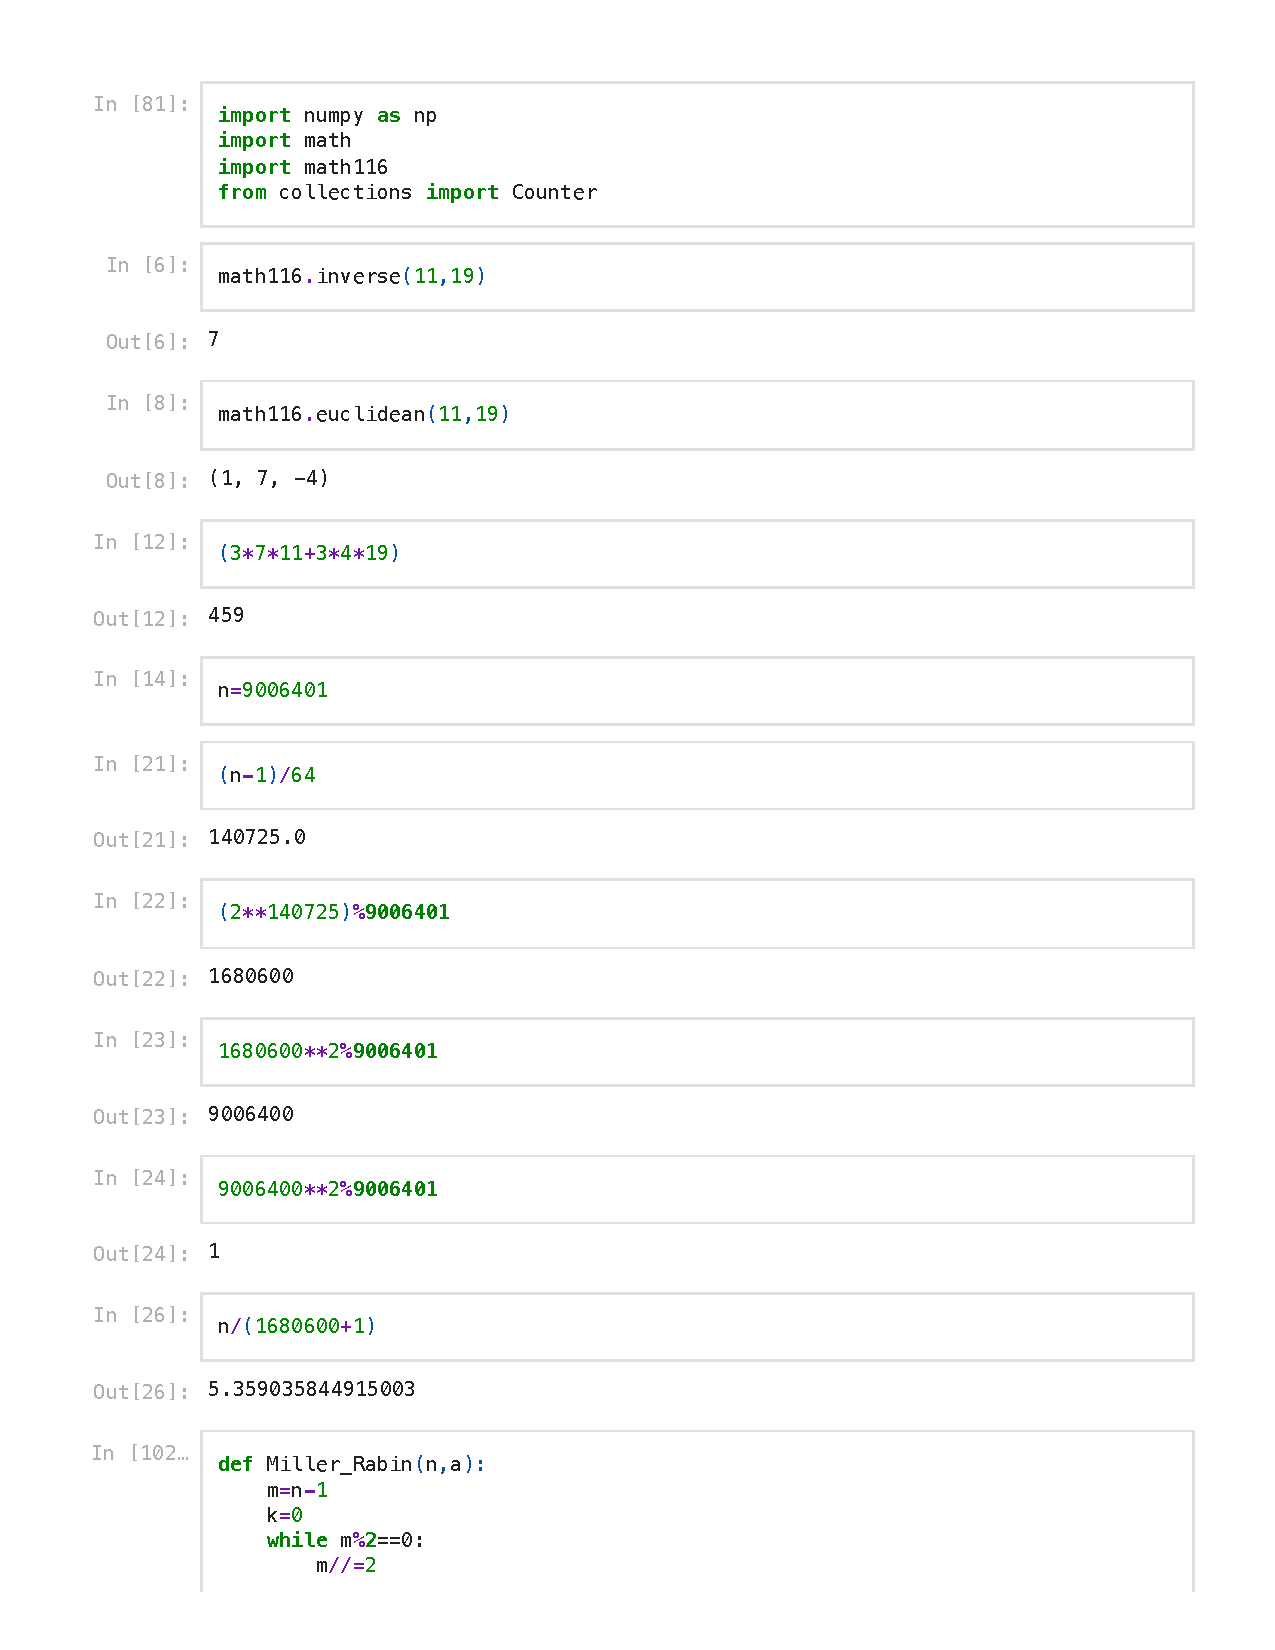
\includepdf[pages=-]{Untitled3.pdf}
\end{enumerate}
\end{document}